\section*{4.1. Mô hình cây quyết định}

Dùng logarithm nhị phân trong entropy: \(\log\) hiểu là \(\log_2\).
Ký hiệu \(H(S)\) là entropy của tập nhãn của \(S\) (theo các lớp xuất hiện trong \(S\)).

%--------------------------------------------------------------------
\subsection*{Câu 4.1.1. Dự đoán mùa trong năm}

\textbf{Dữ liệu huấn luyện (12 mẫu) và hai mẫu cần dự báo \(X\), \(Y\).}

\begin{center}
{\small
\begin{tabular}{@{}ccccc@{}}\toprule
Mẫu & Thời tiết & Lá cây & Nhiệt độ & Mùa\\\midrule
1 & Nắng & Vàng & Trung bình & Thu\\
2 & Tuyết & Xanh & Thấp & Đông\\
3 & Tuyết & Vàng & Thấp & Đông\\
4 & Mưa & Vàng & Trung bình & Thu\\
5 & Mưa & Rụng & Thấp & Đông\\
6 & Tuyết & Rụng & Thấp & Đông\\
7 & Nắng & Rụng & Thấp & Đông\\
8 & Nắng & Xanh & Trung bình & Xuân\\
9 & Nắng & Xanh & Cao & Hè\\
10 & Mưa & Rụng & Trung bình & Thu\\
11 & Mưa & Xanh & Cao & Hè\\
12 & Mưa & Xanh & Trung bình & Xuân\\
\(X\) & Mưa & Vàng & Thấp & ?\\
\(Y\) & Tuyết & Rụng & Trung bình & ?\\
\bottomrule
\end{tabular}
}
\end{center}

\subsubsection*{(a) Thuật toán ID3 (entropy --- Information Gain)}

\textbf{Bước 1 --- Lần chia đầu (trên cả 12 mẫu).}

Tần số nhãn: Thu (3), Đông (5), Xuân (2), Hè (2).
\[
H(S)= -\tfrac{3}{12}\log\tfrac{3}{12}-\tfrac{5}{12}\log\tfrac{5}{12}
      -2\cdot\tfrac{2}{12}\log\tfrac{2}{12}
      \approx 1{,}8879.
\]

Với mỗi thuộc tính, tính entropy có trọng số sau khi tách theo \emph{tất cả} giá trị của thuộc tính đó, rồi lấy \(\text{Gain}=H(S)-H_{\text{sau tách}}\).

\emph{Thời tiết.} Các nhánh Nắng (4 mẫu), Tuyết (3 mẫu), Mưa (5 mẫu) cho entropy từng nhánh lần lượt khoảng \(2{,}0000\); \(0\); \(1{,}9219\). Trung bình có trọng số
\[
H_{\text{thời tiết}}\approx 1{,}4675,\qquad \text{Gain}\approx 0{,}4204.
\]

\emph{Lá cây.} Nhánh Vàng (3 mẫu), Xanh (5 mẫu), Rụng (4 mẫu) cho
\[
H_{\text{lá}}\approx 1{,}1341,\qquad \text{Gain}\approx 0{,}7538.
\]

\emph{Nhiệt độ.} Nhánh Trung bình (5), Thấp (5), Cao (2): hai nhánh Thấp và Cao thuần nhất (entropy \(0\)); nhánh Trung bình có \(3\) Thu và \(2\) Xuân nên entropy khoảng \(0{,}9710\). Vậy
\[
H_{\text{nhiệt độ}}
=\tfrac{5}{12}\,H_{\text{(Trung bình)}}+\tfrac{5}{12}\cdot 0+\tfrac{2}{12}\cdot 0
\approx 0{,}4046,\qquad \text{Gain}\approx 1{,}4834.
\]

Thuộc tính có gain lớn nhất là \textbf{Nhiệt độ} --- chọn làm nút gốc.

\textbf{Bước 2 --- Các lá trực tiếp từ gốc.}
\begin{itemize}\setlength\itemsep{0pt}
  \item Nhiệt độ \(=\) \textbf{Cao}: hai mẫu 9 và 11 đều là Hè \(\Rightarrow\) \textbf{Hè}.
  \item Nhiệt độ \(=\) \textbf{Thấp}: toàn nhãn Đông \(\Rightarrow\) \textbf{Đông}.
  \item Nhiệt độ \(=\) \textbf{Trung bình}: còn 5 mẫu (1,4,8,10,12) với nhãn Thu--Thu--Xuân--Thu--Xuân.
\end{itemize}

\textbf{Bước 3 --- Lần chia trên nhánh «Trung bình».}

Gọi \(S'=\) tập \(5\) mẫu trên. \(H(S')=-\tfrac{3}{5}\log\tfrac{3}{5}-\tfrac{2}{5}\log\tfrac{2}{5}\approx 0{,}9710\).

\emph{Thuộc tính «Thời tiết».} Trong \(S'\) không có thời tiết Tuyết. Nhánh Nắng gồm (1, Thu) và (8, Xuân). Nhánh Mưa gồm (4, Thu), (10, Thu), (12, Xuân). Entropy có trọng số \(\approx 0{,}9510\); Gain \(\approx 0{,}020\).

\emph{Thuộc tính «Lá cây»:} nhánh «Vàng» gồm (1Thu, 4Thu); «Xanh» gồm (8Xuân,12Xuân); «Rụng» gồm (10Thu) --- đều thuần nhất, entropy từng nhánh là \(0\). Vậy \(H_{\text{sau tách}}=0\), \(\text{Gain}\approx 0{,}9710\).

Chọn \textbf{Lá cây} trong nhánh này.

\textbf{Cây thu được (mô tả bằng luật if--then).}
\begin{enumerate}\setlength\itemsep{0pt}
  \item Nếu Nhiệt độ \(=\) Cao \(\Rightarrow\) Hè.
  \item Nếu Nhiệt độ \(=\) Thấp \(\Rightarrow\) Đông.
  \item Nếu Nhiệt độ \(=\) Trung bình và Lá cây \(=\) Xanh \(\Rightarrow\) Xuân.
  \item Nếu Nhiệt độ \(=\) Trung bình và (Lá cây \(=\) Vàng hoặc Rụng) \(\Rightarrow\) Thu.
\end{enumerate}

\begin{center}
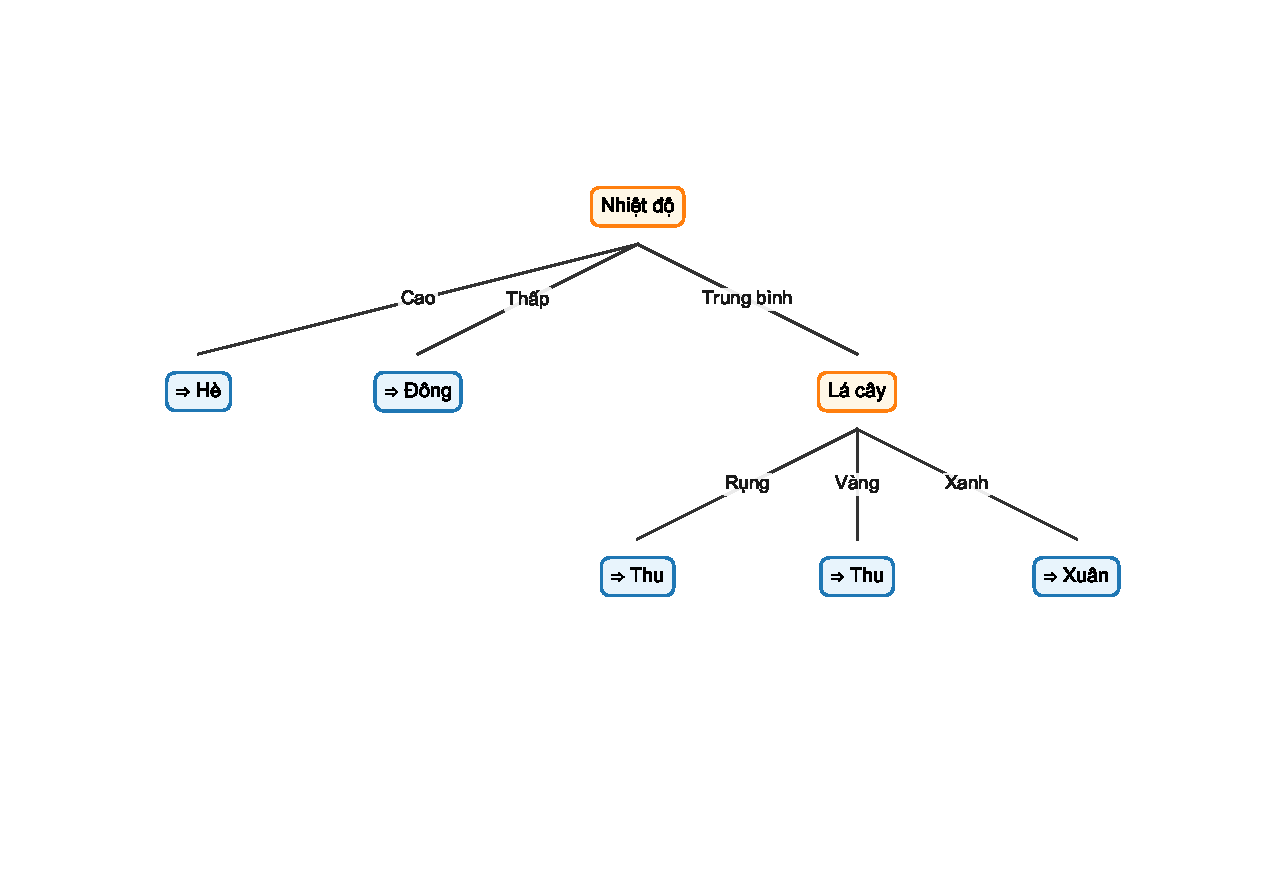
\includegraphics[width=0.96\textwidth]{figures/tree_411_muas_entropy.pdf}\\[4pt]
\small\textit{Minh họa cấu trúc cây theo entropy ở phần (a).}
\end{center}

\subsubsection*{(b) Dự báo \(X\) và \(Y\)}

\begin{itemize}\setlength\itemsep{0pt}
  \item \(X\): (Mưa, Vàng, Thấp) --- theo luật (2) \(\Rightarrow\) \textbf{Đông}.
  \item \(Y\): (Tuyết, Rụng, Trung bình) --- theo luật (4) \(\Rightarrow\) \textbf{Thu}.
\end{itemize}

\subsubsection*{(c) Gini và lỗi phân loại}

Với cùng cách tách đa nhánh như trên, trên bộ 12 mẫu này cả ba tiêu chí (entropy, Gini, lỗi phân loại) đều chọn cùng thứ tự thuộc tính: \textbf{Nhiệt độ} ở gốc, rồi \textbf{Lá cây} trên nhánh «Trung bình»; dự báo \(X\), \(Y\) vẫn là \textbf{Đông} và \textbf{Thu}. Cấu trúc cây minh họa trùng nhau giữa ba tiêu chí (có thể vẽ riêng nếu cần đối chiếu hình).

%--------------------------------------------------------------------
\subsection*{Câu 4.1.2. Độc / không độc của lá (10 mẫu học)}

\textbf{Dữ liệu (Huấn luyện: 1--10; kiểm tra: 11, 12.)}

\begin{center}
{\footnotesize
\begin{tabular}{@{}cccccc@{}}\toprule
Mẫu & Hình dạng & Dạng & Màu & Kích thước & Độc\\\midrule
1 & Tròn & Đơn & Đỏ & Nhỏ & Không\\
2 & Tròn & Kép & Đỏ & Nhỏ & Có\\
3 & Tròn & Đơn & Xanh & To & Không\\
4 & Dài & Đơn & Xanh & Nhỏ & Không\\
5 & Dài & Kép & Vàng & Nhỏ & Có\\
6 & Dài & Đơn & Xanh & Vừa & Có\\
7 & Tròn & Kép & Vàng & To & Không\\
8 & Tròn & Kép & Vàng & Vừa & Có\\
9 & Tròn & Đơn & Đỏ & Vừa & Có\\
10 & Dài & Đơn & Đỏ & Vừa & Có\\
11 & Dài & Kép & Đỏ & Vừa & ?\\
12 & Tròn & Đơn & Xanh & Nhỏ & ?\\
\bottomrule
\end{tabular}
}
\end{center}

Trên \(10\) mẫu, Không và Có có tần \(4\) và \(6\). Entropy gốc
\[
H(S)=-\tfrac{4}{10}\log\tfrac{4}{10}-\tfrac{6}{10}\log\tfrac{6}{10}\approx 0{,}9710.
\]

\subsubsection*{(a) Theo chỉ số Gini --- lần đầu}

Gini của tập: \(i(S)=1-\bigl(\tfrac{4}{10}\bigr)^2-\bigl(\tfrac{6}{10}\bigr)^2=0{,}48\).

Tách theo \textbf{Kích thước}: nhánh ``Nhỏ'' gồm bốn mẫu 1--2--4--5 với nhãn lần lượt Không, Có, Không, Có; nhánh ``To'' một mẫu Không; nhánh ``Vừa'' ba mẫu đều Có.
Impurity Gini từng nhánh: ``Nhỏ'' là \(1-(\tfrac{2}{4})^2-(\tfrac{2}{4})^2=\tfrac{1}{2}\); ``To'' và ``Vừa'' bằng \(0\) (thuần nhất). Gini có trọng số:
\[
\textstyle \tfrac{4}{10}\cdot 0{,}5+\tfrac{1}{10}\cdot 0+\tfrac{3}{10}\cdot 0=0{,}20,\qquad \Delta\approx 0{,}28
\]
lớn nhất so với các thuộc tính còn lại (Đối chiếu khi tính tay: ``Màu'' có Gini có trọng số \(\approx 0{,}4167\), ``Hình dạng'' và ``Dạng'' có Gini có trọng số \(\approx 0{,}45\)). Vậy chọn \textbf{Kích thước} ở gốc.

\subsubsection*{Nhánh «Kích thước \(=\) Nhỏ»}

Bốn mẫu còn lại có nhãn Không--Có--Không--Có (entropy \(1\)). Tách theo \textbf{Dạng}: «Đơn» (2 Không), «Kép» (2 Có) --- thuần nhất. Đây là lần chia thứ hai.

Nhánh «To» và «Vừa» đã thuần «Không» và «Có».

\begin{center}
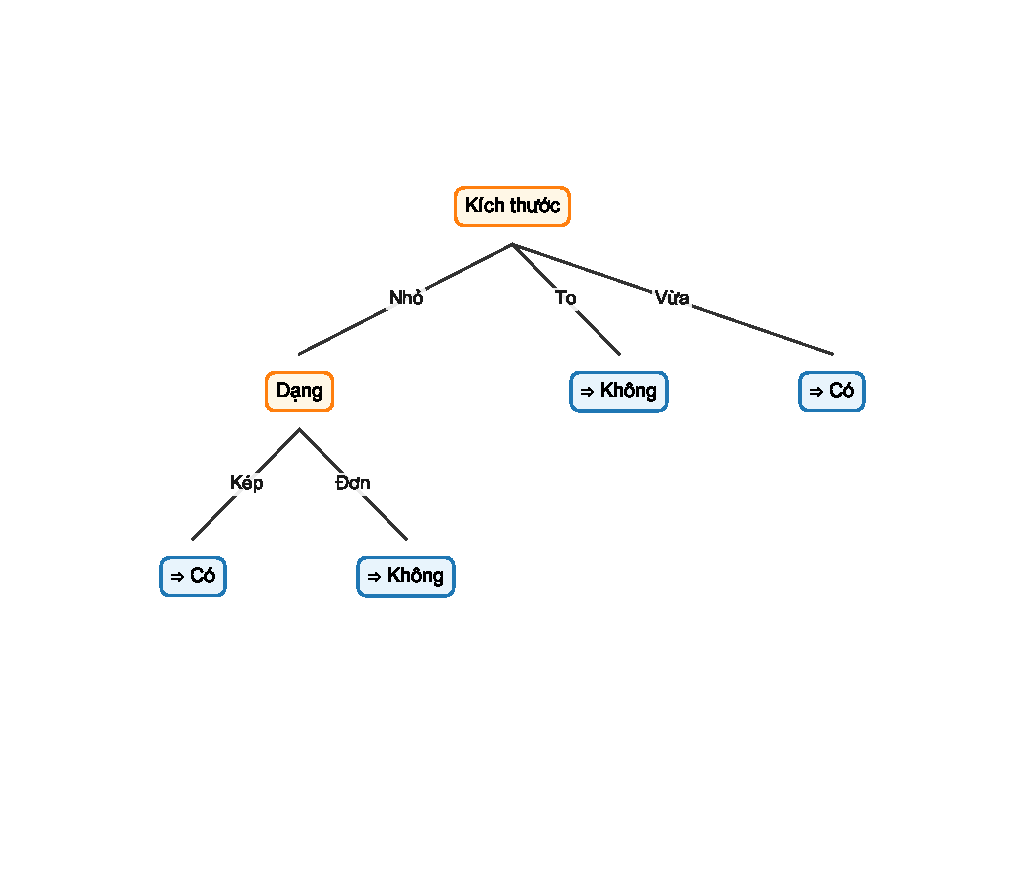
\includegraphics[width=0.96\textwidth]{figures/tree_412_la_gini.pdf}\\[4pt]
\small\textit{Minh họa cây theo Gini như phần (a).}
\end{center}

\subsubsection*{(b) Dự báo mẫu 11 và 12}

Theo cây tìm được:
\begin{itemize}\setlength\itemsep{0pt}
  \item Mẫu 11 (Dài, Kép, Đỏ, Vừa): Kích thước ``Vừa'' \(\Rightarrow\) \textbf{Có}.
  \item Mẫu 12 (Tròn, Đơn, Xanh, Nhỏ): ``Nhỏ'' rồi ``Đơn'' \(\Rightarrow\) \textbf{Không}.
\end{itemize}

\subsubsection*{(c) Entropy và lỗi phân loại}

Ở gốc, entropy có trọng số sau khi tách theo Kích thước là \(0{,}4000\) (gain \(0{,}5709\)), lớn hơn các thuộc tính khác; lỗi phân loại có trọng số cũng đạt cực tiểu \(0{,}20\) với cùng thuộc tính \textbf{Kích thước}. Bước kế trên nhánh «Nhỏ» vẫn chọn \textbf{Dạng}. Kết quả dự báo mẫu 11, 12 trùng phần (a)--(b): \textbf{Có} và \textbf{Không}.

%--------------------------------------------------------------------
\subsection*{Câu 4.1.3. Quyết định cho vay (10 mẫu học)}

\textbf{Dữ liệu.}

\begin{center}
{\footnotesize
\begin{tabular}{@{}cccccc@{}}\toprule
Mẫu & Phái & Công việc & Học vấn & Độ tuổi & Quyết định\\\midrule
1 & Nam & LĐ Chân tay & Cao đẳng & Trung niên & Không\\
2 & Nữ & LĐ Trí óc & Đại học & Trung niên & Có\\
3 & Nữ & LĐ Chân tay & Phổ thông & Già & Có\\
4 & Nam & LĐ Trí óc & Cao đẳng & Trung niên & Có\\
5 & Nam & LĐ Chân tay & Phổ thông & Thanh niên & Không\\
6 & Nam & LĐ Trí óc & Đại học & Già & Có\\
7 & Nam & LĐ Chân tay & Cao đẳng & Già & Có\\
8 & Nữ & LĐ Chân tay & Phổ thông & Trung niên & Không\\
9 & Nam & LĐ Trí óc & Đại học & Thanh niên & Không\\
10 & Nữ & LĐ Chân tay & Cao đẳng & Già & Có\\
A & Nữ & LĐ Trí óc & Cao đẳng & Già & ?\\
B & Nam & LĐ Chân tay & Phổ thông & Trung niên & ?\\
\bottomrule
\end{tabular}
}
\end{center}

\subsubsection*{(a) Lỗi phân loại}

Tại gốc, lỗi gốc \(=1-\max(\tfrac{4}{10},\tfrac{6}{10})=0{,}40\).
Tách theo \textbf{Độ tuổi}: Già (4 mẫu toàn «Có»), Thanh niên (2 mẫu toàn «Không»), Trung niên (4 mẫu: hai Không và hai Có---lỗi impurity của nút bằng \(1-\tfrac{2}{4}=0{,}5\)). Lỗi có trọng số
\[
\tfrac{4}{10}\cdot 0+\tfrac{2}{10}\cdot 0+\tfrac{4}{10}\cdot 0{,}5=0{,}20,
\]
giảm nhiều nhất so với Phái, Công việc (lỗi có trọng số \(0{,}40\) tại nút đầu) và Học vấn (\(0{,}30\)). Chọn \textbf{Độ tuổi} gốc.

Trên nhánh Trung niên, tách tiếp theo \textbf{Công việc}: hai nhánh đều thuần (Chân tay \(\to\) Không; Trí óc \(\to\) Có).

Luật (tóm tắt):
\begin{enumerate}\setlength\itemsep{0pt}
  \item Độ tuổi \(=\) Già \(\Rightarrow\) Có.
  \item Độ tuổi \(=\) Thanh niên \(\Rightarrow\) Không.
  \item Độ tuổi \(=\) Trung niên và công việc thuộc nhóm trí óc \(\Rightarrow\) Có.
  \item Độ tuổi \(=\) Trung niên và công việc chân tay \(\Rightarrow\) Không.
\end{enumerate}

\begin{center}
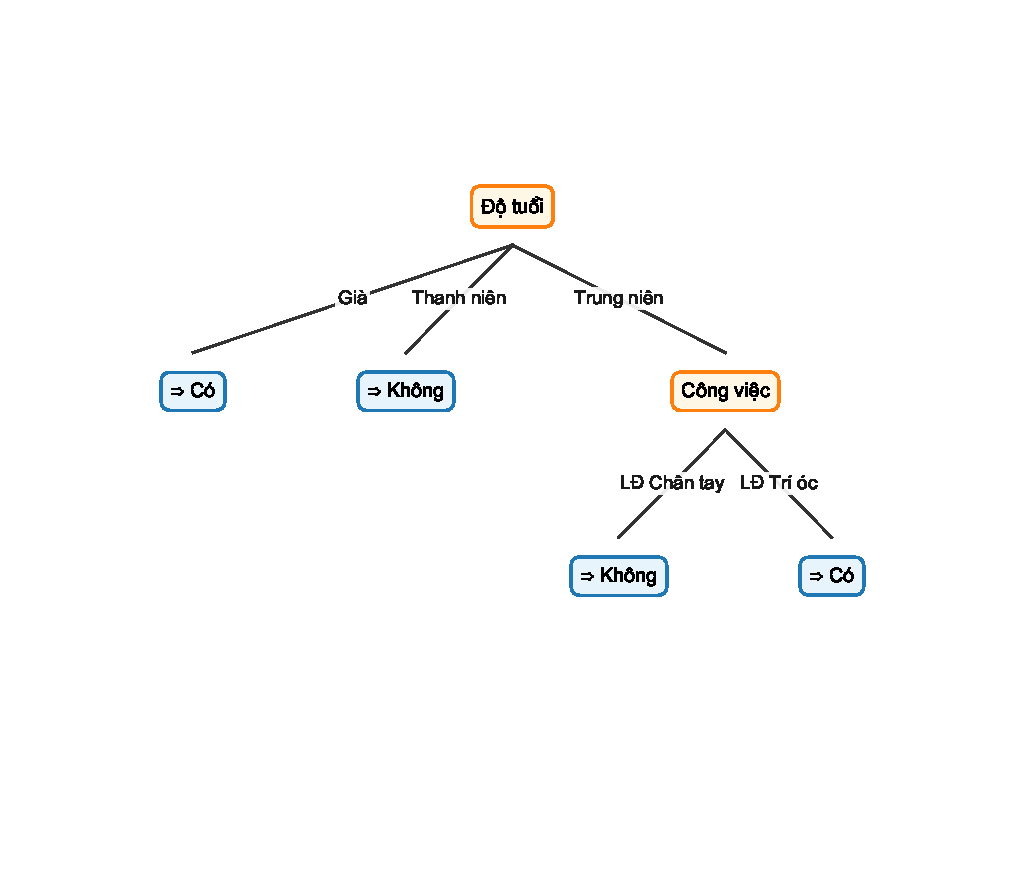
\includegraphics[width=0.96\textwidth]{figures/tree_413_vay_error.pdf}\\[4pt]
\small\textit{Minh họa cây theo lỗi phân loại ở phần (a).}
\end{center}

\subsubsection*{(b) Dự báo A và B}

\begin{itemize}\setlength\itemsep{0pt}
  \item A (Nữ, Trí óc, Cao đẳng, Già): theo luật (1) \(\Rightarrow\) \textbf{Có}.
  \item B (Nam, Chân tay, Phổ thông, Trung niên): luật (4) \(\Rightarrow\) \textbf{Không}.
\end{itemize}

\subsubsection*{(c) Gini và entropy}

Entropy gốc bằng \(0{,}9710\) (nhãn \(4/10\) và \(6/10\)).

Tại gốc, entropy có trọng số sau khi tách theo Độ tuổi là \(0{,}4000\) (gain \(0{,}5709\)), lớn nhất; Gini có trọng số \(0{,}2000\) (độ giảm \(0{,}2800\)) cũng đạt cực đại. Bước kế trên «Trung niên» vẫn chọn \textbf{Công việc}. Dự báo A, B giữ nguyên \textbf{Có} và \textbf{Không}.

%--------------------------------------------------------------------
\subsection*{Câu 4.1.4. Hồ sơ vay vốn (C4.5 --- Information Gain)}

Trên tập chỉ gồm thuộc tính phân loại, ta dùng Information Gain (entropy \(\log_2\)) để chọn thuộc tính tách tại mỗi nút (cùng cách tách đa nhánh như ID3).

\textbf{Dữ liệu (15 mẫu).}

\begin{center}
{\footnotesize
\begin{tabular}{@{}cccccc@{}}\toprule
Mẫu & Age & Has\_job & Own\_house & Credit\_rating & Class\\\midrule
1 & young & false & false & fair & No\\
2 & young & false & false & good & No\\
3 & young & true & false & good & Yes\\
4 & young & true & true & fair & Yes\\
5 & young & false & false & fair & No\\
6 & middle & false & false & fair & No\\
7 & middle & false & false & good & No\\
8 & middle & true & true & good & Yes\\
9 & middle & false & true & excellent & Yes\\
10 & middle & false & true & excellent & Yes\\
11 & old & false & true & excellent & Yes\\
12 & old & false & true & good & Yes\\
13 & old & true & false & good & Yes\\
14 & old & true & false & excellent & Yes\\
15 & old & false & false & fair & No\\
\bottomrule
\end{tabular}
}
\end{center}

\subsubsection*{(a) Xây cây theo Information Gain}

Tại gốc: các nhãn ``No'' và ``Yes'' có tần \(6\) và \(9\) (trên \(15\) mẫu). Entropy
\[
H(S)=-\tfrac{6}{15}\log\tfrac{6}{15}-\tfrac{9}{15}\log\tfrac{9}{15}\approx 0{,}9710.
\]

Tính entropy có trọng số sau khi tách theo từng thuộc tính (mỗi thuộc tính tách theo \emph{tất cả} giá trị của nó), rồi \(\text{Gain}=H(S)-H_{\text{sau tách}}\). Kết quả so sánh (làm tròn):
\begin{itemize}\setlength\itemsep{0pt}
  \item \texttt{Own\_house}: \(H_{\text{sau}}\approx 0{,}5510\), \(\text{Gain}\approx 0{,}4200\) (lớn nhất).
  \item \texttt{Credit\_rating}: \(H_{\text{sau}}\approx 0{,}6080\), \(\text{Gain}\approx 0{,}3630\).
  \item \texttt{Has\_job}: \(H_{\text{sau}}\approx 0{,}6473\), \(\text{Gain}\approx 0{,}3237\).
  \item \texttt{Age}: \(H_{\text{sau}}\approx 0{,}8879\), \(\text{Gain}\approx 0{,}0830\).
\end{itemize}

Vậy nút gốc là \textbf{\texttt{Own\_house}}.

\medskip
\noindent\emph{Nhánh \texttt{Own\_house} \(=\) true.} Có \(6\) mẫu (4,8,9,10,11,12) và tất cả đều ``Yes'' \(\Rightarrow\) lá nhãn \textbf{Yes}.

\medskip
\noindent\emph{Nhánh \texttt{Own\_house} \(=\) false.} Còn \(9\) mẫu với \(6\) ``No'' và \(3\) ``Yes'':
\[
H(S')=-\tfrac{6}{9}\log\tfrac{6}{9}-\tfrac{3}{9}\log\tfrac{3}{9}\approx 0{,}9183.
\]
So sánh gain trên các thuộc tính còn lại (\texttt{Age}, \texttt{Has\_job}, \texttt{Credit\_rating}): \texttt{Has\_job} cho các nhánh thuần nhất (``false'': toàn ``No''; ``true'': toàn ``Yes''), entropy sau tách bằng \(0\) nên \(\text{Gain}\approx 0{,}9183\) --- lớn nhất. Chọn \textbf{\texttt{Has\_job}} tại nút này.

Cây thu được có dạng sau (minh họa bằng hình):

\begin{center}
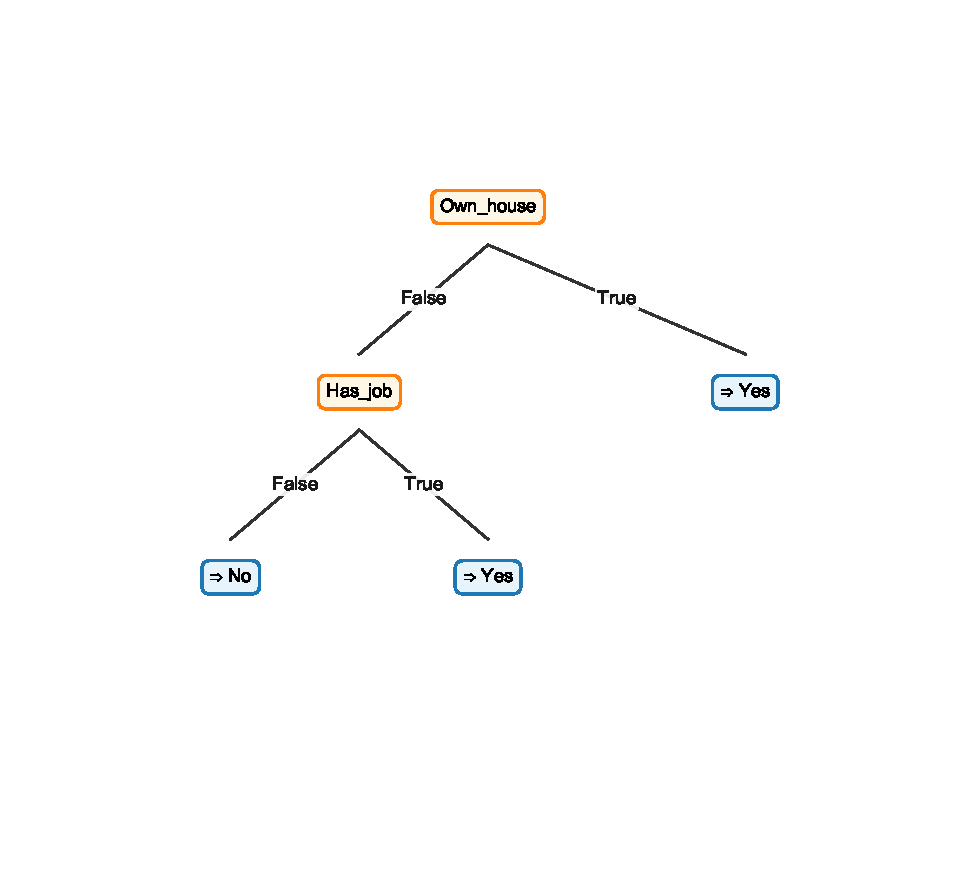
\includegraphics[width=0.96\textwidth]{figures/tree_414_loan_ig.pdf}\\[4pt]
\small\textit{Cây theo Information Gain (entropy).}
\end{center}

\subsubsection*{(b) Luật quyết định (if--then)}

Từ cây ở phần (a), có thể viết gọn:
\begin{enumerate}\setlength\itemsep{0pt}
  \item Nếu \texttt{Own\_house} \(=\) true thì \textbf{Yes}.
  \item Nếu \texttt{Own\_house} \(=\) false và \texttt{Has\_job} \(=\) false thì \textbf{No}.
  \item Nếu \texttt{Own\_house} \(=\) false và \texttt{Has\_job} \(=\) true thì \textbf{Yes}.
\end{enumerate}
(Tên thuộc tính giữ như trong đề.)
